\documentclass[bibtotocnumbered, headsepline,normalheadings]{report}
\usepackage[utf8]{inputenc}
\usepackage{color}
\usepackage{tabularx}
\usepackage[T1]{fontenc}
\usepackage{textcomp}
\usepackage[polutonikogreek,english]{babel}
\usepackage{ucs}
\usepackage{booktabs}
\usepackage{multirow}
\usepackage{listings}
\lstset{breaklines=true,showstringspaces=false,numbers=left,frame=single,prebreak=\mbox{$\hookleftarrow$}}
\usepackage[hidelinks]{hyperref}
\usepackage[a4paper,margin=2cm]{geometry} 
\usepackage{scrpage}
\usepackage{alltt}
\usepackage{float}
\usepackage{graphicx}
\definecolor{darkblue}{rgb}{0,0,.5}
\hypersetup{pdftex=true, colorlinks=false, breaklinks=true, citecolor=darkblue, linkcolor=darkblue, menucolor=darkblue, pagecolor=darkblue, urlcolor=darkblue,
pdftitle={embeddedLamp - SPI protocol driver for ARM board for Showing WLAN Link Quality},
pdfauthor={Bartholomäus Dedersen, Kamil Wozniak, Simon Wiesmann, Mathias Goehlke},
bookmarks=true,
bookmarksnumbered=true,
bookmarksopen=true,
bookmarksopenlevel=2}
\pagestyle{headings}
\newcommand{\gdir}%
   {\foreignlanguage{polutonikogreek}}
\begin{document}

\author{ 
Bartholomäus Dedersen \\ Fachhochschule Kiel \\ bartholomaeus.dedersen@student.fh-kiel.de \and
Bla \\ FFF \\ FFF@ff.de}

\date{\today} 
\title{SPI protocol driver for Showing WLAN Link Quality} 

\maketitle


\begin{abstract}

    BLABLA

\end{abstract}

\tableofcontents \newpage

\chapter{Introduction}

The main idea behind this project was to use the \textit{Pandaboard} - an embedded development board - to output information on an external device, in this case a LED bar with 40 LED's. The goal was to create the drivers and to be able to use it universally. We wanted to create the possibility to write different applications for this system, without changing anything on the driver level of the \textit{Pandaboard}. 
Examples for so called \textit{User-space} application are measuring the quality of a connected WLAN, measuring the signal strength of a WLAN and also to output the \textit{Load} - CPU usage - of the \textit{Pandaboard}.

\section{Pandaboard}

\begin{figure}[H]
   \centering
   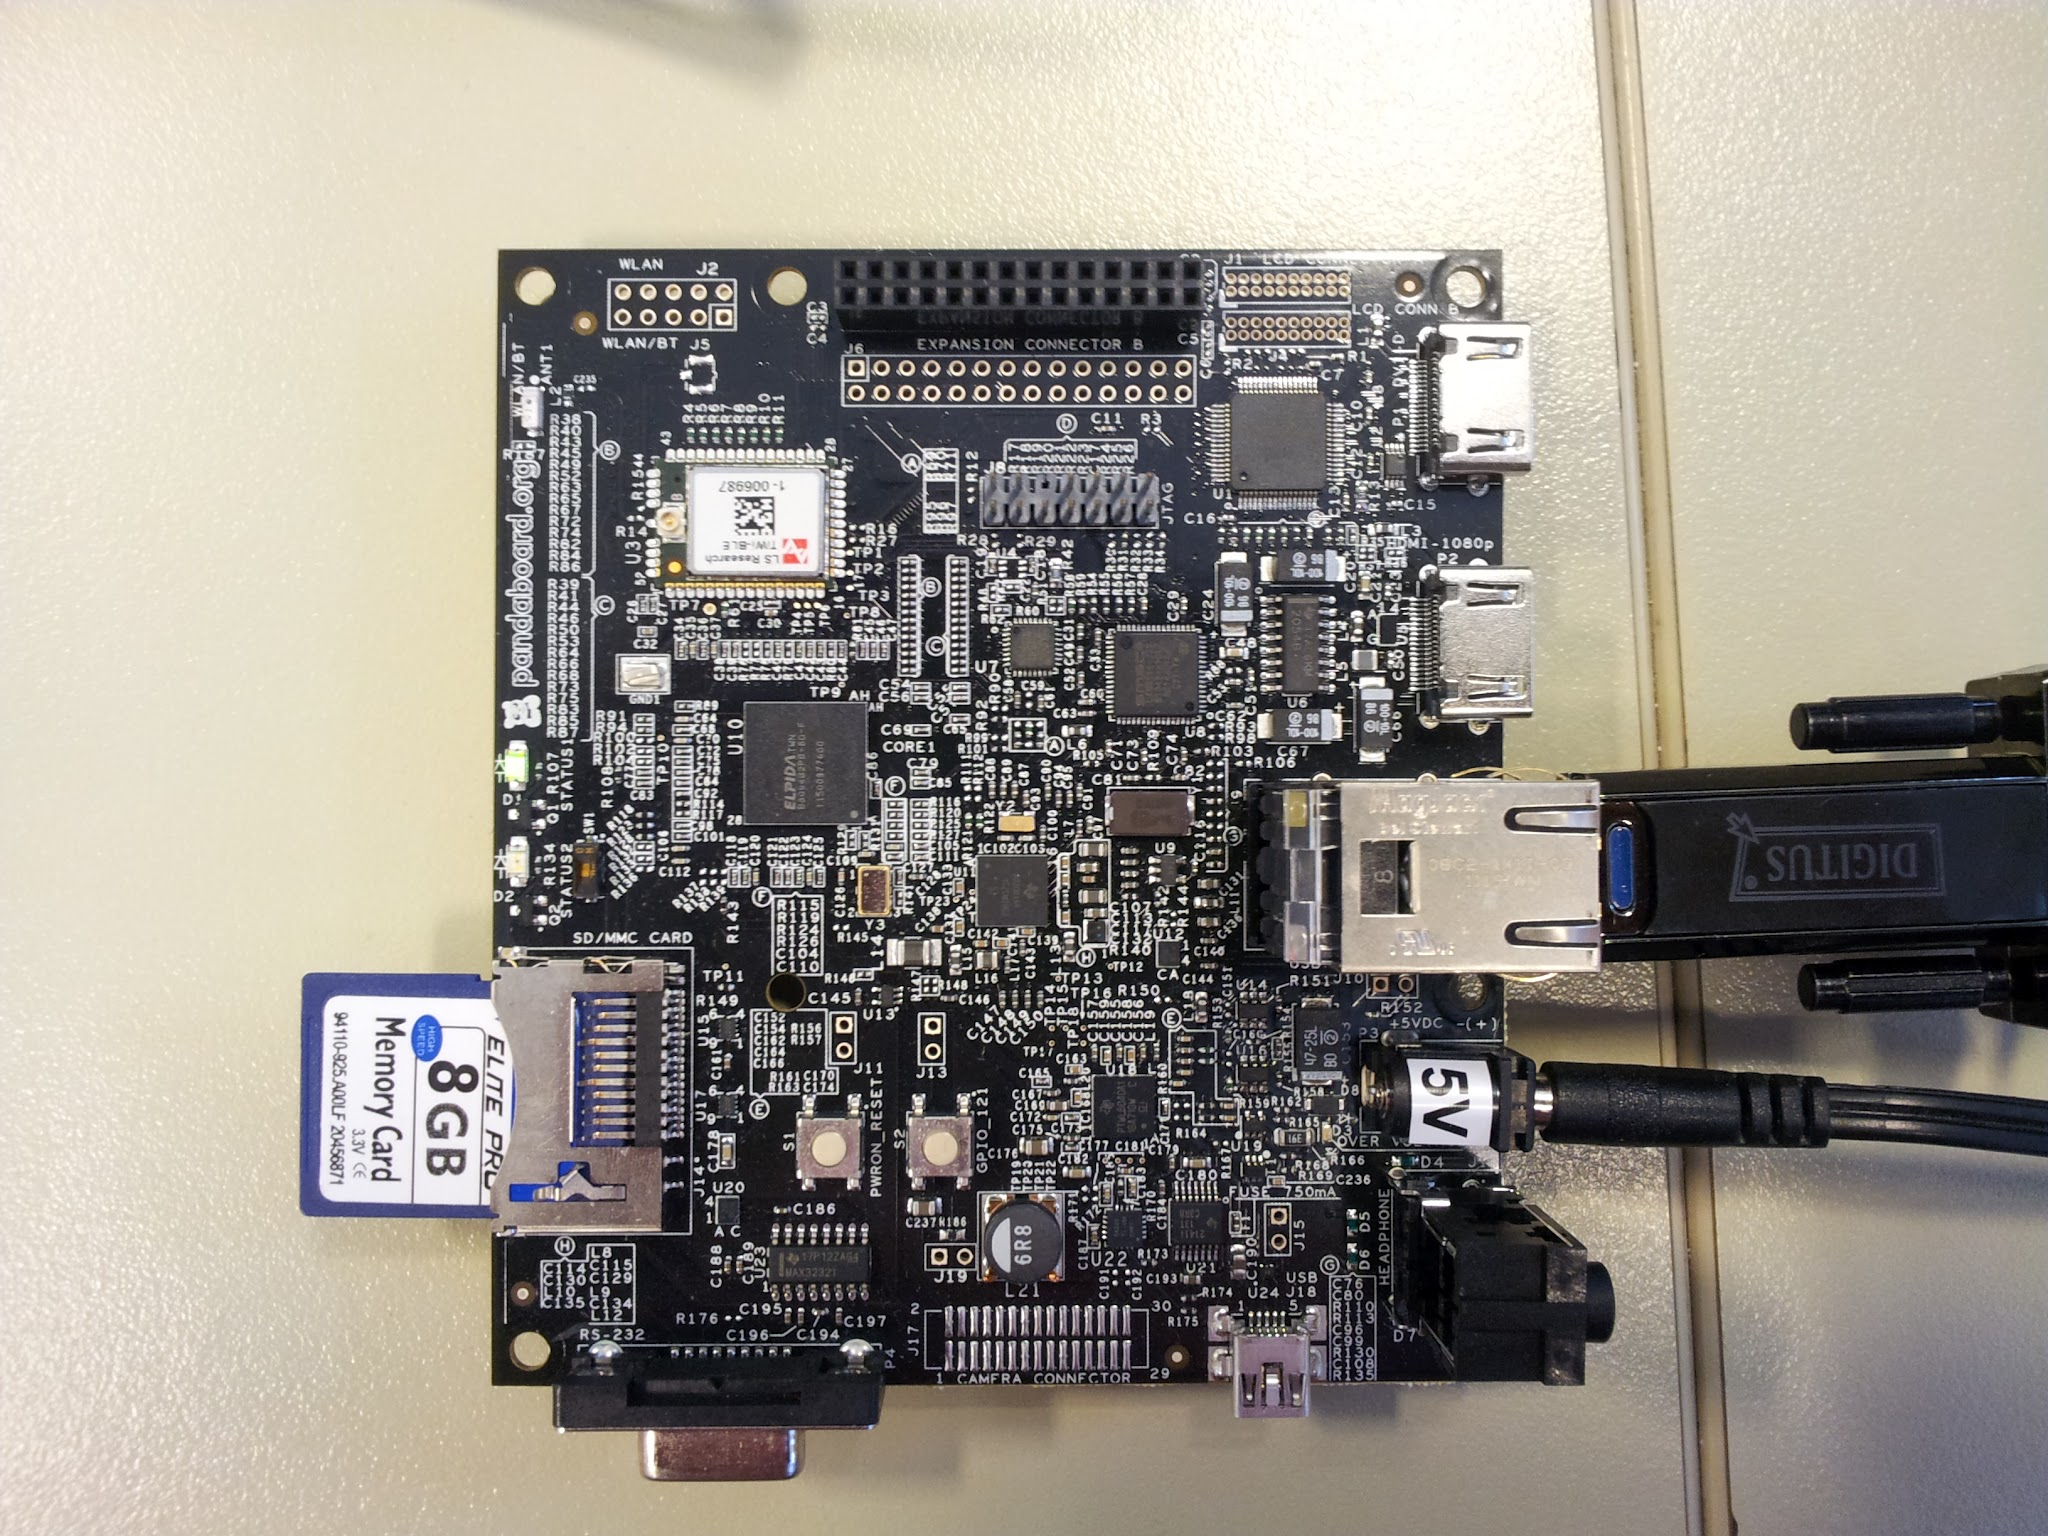
\includegraphics[width=0.8\textwidth]{img/Pandaboard_Alone.jpg}%
   \caption{Pandaboard with installed SD card}
   \label{fig:pandaBoard_Alone}%
\end{figure}

\section{LED-Bar}
\begin{figure}[H]
   \centering
   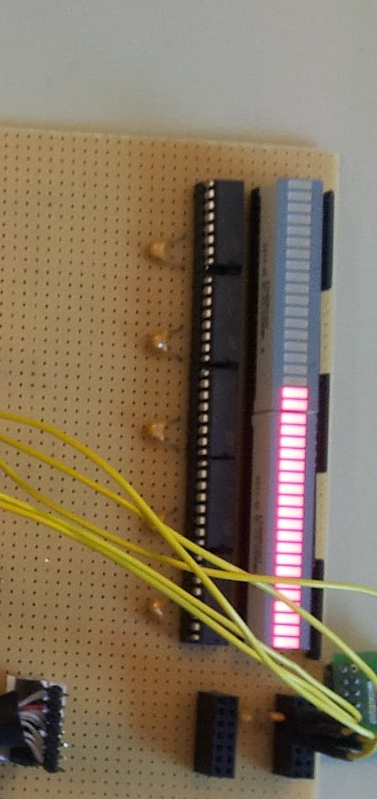
\includegraphics[width=0.3\textwidth]{img/LED-Bar.png}%
   \caption{LED-Bar with 40 LED's and level-shifter.}
   \label{fig:ledBar}%
\end{figure}

\section{Goal to achieve}
\begin{figure}[H]
   \centering
   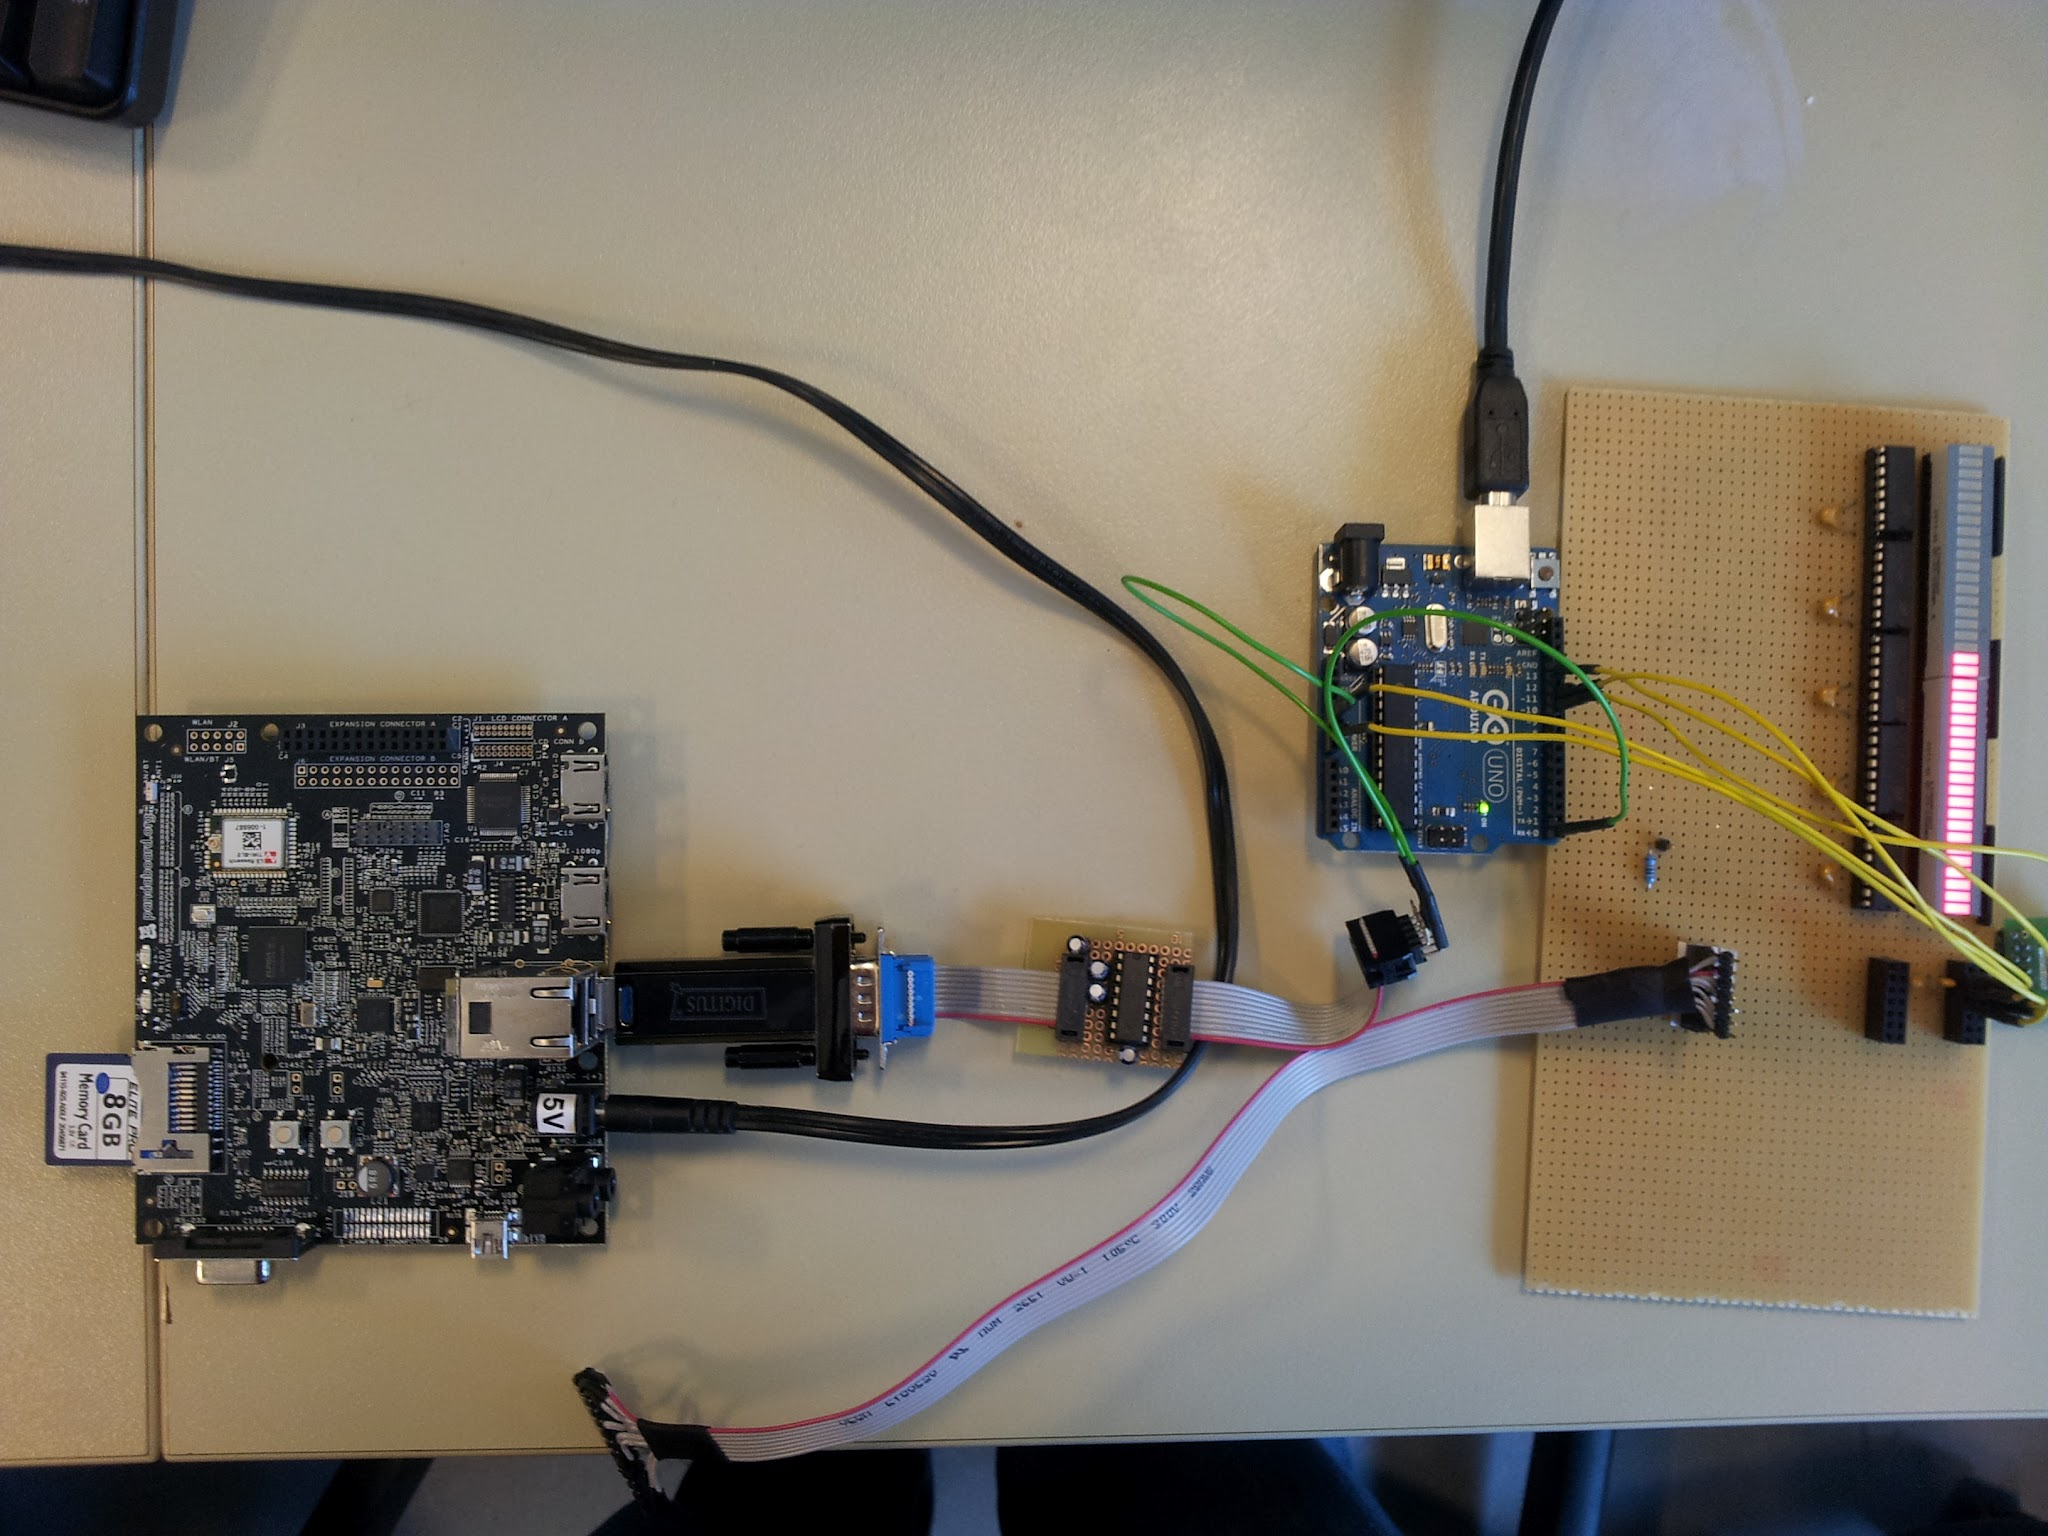
\includegraphics[width=0.8\textwidth]{img/Panda_and_LED_Bar.jpg}%
   \caption{Powering the LED-bar with the Pandaboard and a microcontroller}
   \label{fig:completeProject}%
\end{figure}

\chapter{Hardware Design}
\label{chap:hardware}

\begin{figure}[H]
   \centering
   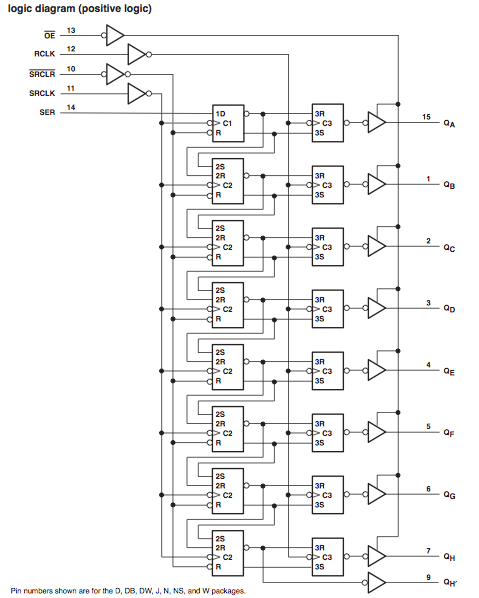
\includegraphics[width=0.5\textwidth]{img/Shift_register.png}%
   \caption{Shift register, source \url{http://www.ti.com/lit/ds/symlink/cd74hc595.pdf}}
   \label{fig:shiftRegister}%
\end{figure}


\begin{figure}[H]
   \centering
   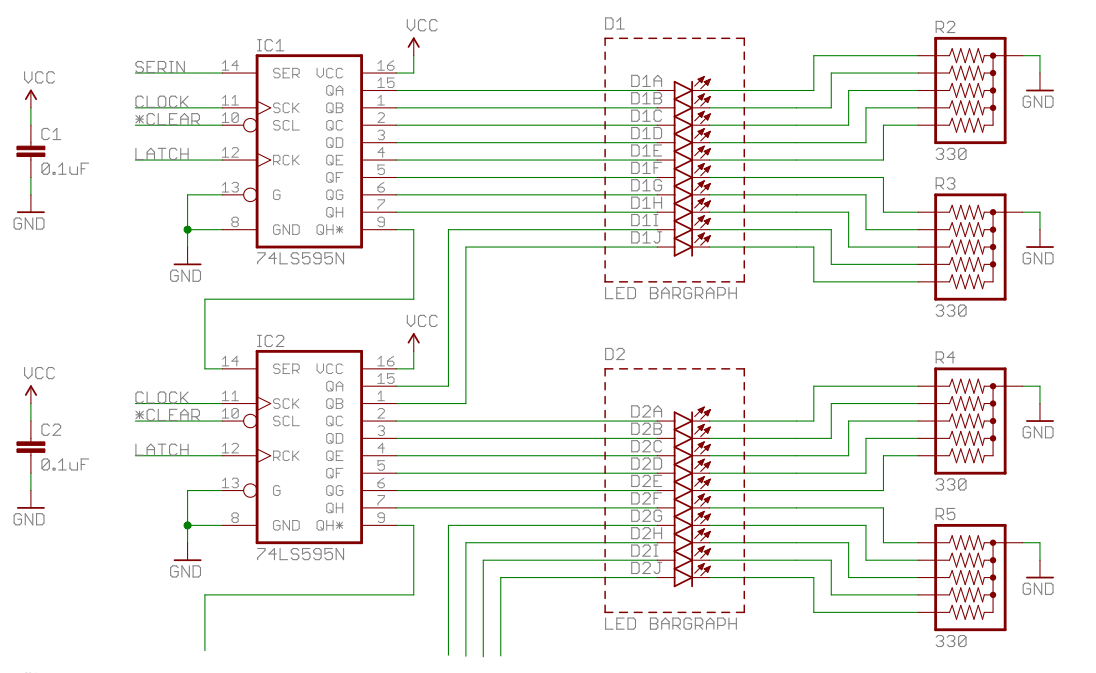
\includegraphics[width=0.8\textwidth]{img/Breakout.png}%
   \caption{Source \url{http://dlnmh9ip6v2uc.cloudfront.net/datasheets/BreakoutBoards/Bargraph Breakout v10.pdf}}
   \label{fig:breakout}%
\end{figure}


\begin{figure}[H]
   \centering
   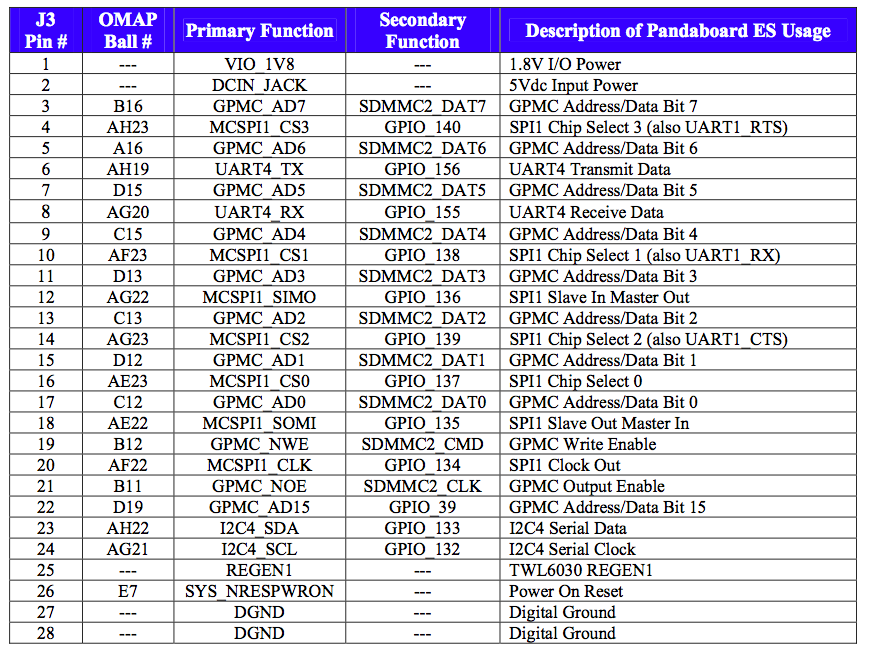
\includegraphics[width=0.8\textwidth]{img/PandaBoard_IO_J3.png}%
   \caption{Pandaboard IO J3 connectors,  source  \url{http://pandaboard.org/sites/default/files/board_reference/ES/Panda_Board_Spec_DOC-21054_REV0_1.pdf}}
   \label{fig:pandaBoardIOJ3}%
\end{figure}

\begin{figure}[H]
   \centering
   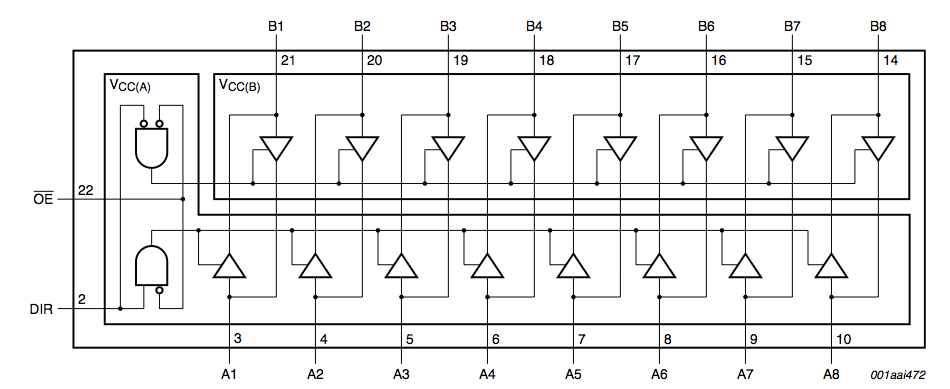
\includegraphics[width=0.8\textwidth]{img/level_Shifter.png}%
   \caption{Level shifter, source NXP  74LVC8T245 Manual}
   \label{fig:level_Shifter}%
\end{figure}

\begin{figure}[H]
   \centering
   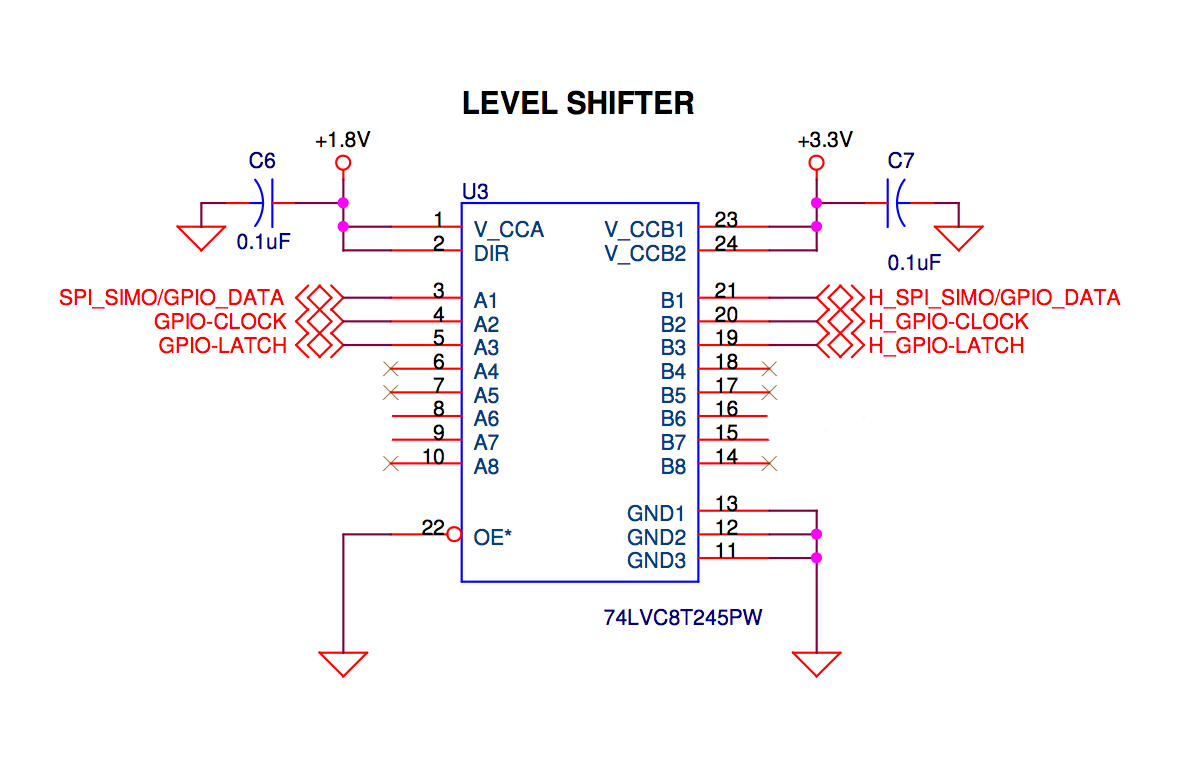
\includegraphics[width=0.8\textwidth]{img/Levelshifter.png}%
   \caption{Level Shifter}
   \label{fig:levelShifter2}%
\end{figure}

\chapter{Kernel Interface}
\label{chap:kernel}
\section{Reasons for SPI}

Choices fell on SPI. Alternatives before taking the choice were:

\begin{description}
\item[\(GPIO\)] The Panda Board offer multiple pins which can be either controlled with userspace or kernelspace commands. Speed is not determined by official 
instructions but below SPI bus speed.\footnote{\url{https://groups.google.com/forum/\#!msg/pandaboard/mqfaT54NzWk/UH5HIhlg\_TsJ}}
\item[\(I^2C\)] Various pins available. Choice number 2 for the project.
\item[\(Serial Port\)] One connector available but used for debugging. Speed is measured in baud.
\item[\(SPI\)] Multiple pins on both expansion connectors available. Speed successfully tested up to 10 MHz.
\end{description}

Main reason for the group's choice was the speed and the educational effect of appling a SPI implementation to an ARM-Board.

An oscilloscope was used for debugging purpose and was needed multiple times.

\section{SPI for Linux}

The SPI interface is documented in \url{http://www.kernel.org/doc/Documentation/spi/spi-summary}. There was no need for a MISO\footnote{Master In, Slave Out} connection as the LED-bar was solely receiving data.
Different clock modes could be used but as the clock was not used in this project altogether to the expense of inability to drive the LED bar in parallel with other SPI slaves.

Two different approaches for programming were available:
\begin{enumerate}
\item spidev is a development driver which is already included in the kernel. It can be used to test SPI functionality but is not as much configurable as a custom protocol driver.
\item SPI protocol drivers allow the whole range of configuration. Some kernel provided structures have to be used.
\end{enumerate}

\subsection{Various Howtos}

The instruction for using the GPIO ports for latching were taken from
\url{http://www.nerdenmeister.org/2011/11/13/using-the-gpio-pins-on-a-pandaboard/} in addition to the official kernel documentation.
The link only provides userspace toggling but similar functionality can be archived by using direct kernel functions as pointed out 
by \url{http://www.kernel.org/doc/Documentation/gpio.txt}.

Most useful for this project is the rather lengthly Howto from Scott Ellis available at \url{http://www.jumpnowtek.com/index.php?option=com\_content&view=article&id=57&Itemid=62}. His tutorial covered the whole development process of an SPI protocol driver and was 
written for the Beagleboard. The author of this project adapted it to the Pandaboard and most of the kernel module code is based on the last
version of Scott's driver. We want to thank the author as his documentation was the only complete one.

\section{Practical Work}

For preparation some necessary header files for compiling a kernel module are required. There is no need for a complete kernel source as 
wrongly pointed out by the Beagleboard-group. As the complete sources for the Texas Instrument kernel are not available the headers 
are the only option. 

The installation in a Debian environment is done by \textsl{sudo apt-get linux-headers-omap4}. The files will be available in the 
directory \textsl{/usr/src}.

Compiling is done with a self-made Makefile which is available in the Github repository. Mainly it specified the location for the header files
and inserts the module if the compilation succeeded. Another option for the makefile is to remove the kernel by one command for increasing 
the handling for other group members.

Practical for visualisation of the source code is an activity diagram as shown in figure~\ref{fig:actKernel}. After the critical 
initialisation part which was encountered in error frequently due to insufficient rights for inserting the module or taking bogus parametres
in the development phase the LED-bar is accessible through a char device called \textsl{/dev/embeddedLamp}. It starts running a counter 
which omits the chip programming specialities and just shifts binary ones beginning from zero. When the total amount of bits for the 
LED is reached it starts from zero again.

Every message which is transmitted over the SPI-bus contains five 8 bit unsigned integers, representing each part of the LED-bar. The 
data is wrapped in a C-structure which interface is given by the Linux kernel. Also, the five messages are part of a transfer structure which 
is finally send over SPI.

\begin{figure}[h]
   \centering
   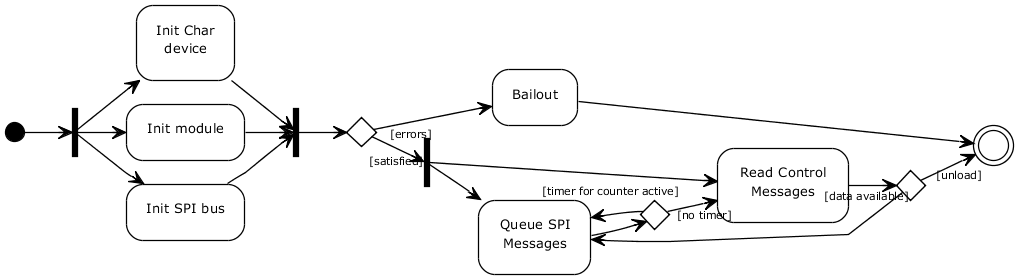
\includegraphics[width=\textwidth]{img/kernel_activity.png}%
   \caption{Activity Diagram for Kernel Module}
   \label{fig:actKernel}%
\end{figure}

One additional interface was included by reading the char device. It displays the total amount of sent counter messages and the amount of 
lost messages. The loss was between 1\% and 0.1\% of total messages, depending and correlating on the bus speed.
An example command would be \textsl{cat /dev/embeddedLamp}.

By sending the command \textsl{start} the counter starts and by sending \textsl{stop} it supposedly should stop. An example command is \textsl{echo 'start' >/dev/embeddedLamp}.

Another way of accessing the LED-bar is by echo'ing the hexadecimal representation to the char device, e.g. \textsl{echo 'DEADBEEF00' >/dev/embeddedLamp}. The kernel driver searches for a ten char long string and lights up the LED. This is exportable for userspace access and was finally used for the WiFi-Quality representation.


\chapter{Userspace Driver}
\label{chap:userspace}
\section{C Application wlan\_info.c}

The initial choice was to write an application in C and use the \textit{iwlib} library provided by the \textit{Wireless Tools} project \footnote{\url{http://www.hpl.hp.com/personal/Jean_Tourrilhes/Linux/Tools.html}}. It is funded by \textit{Hewlett Packard} and available as Open Source software. Furthermore, it also includes applications for getting data about wireless hardware and information about wireless networks.

The application consists of two files: \textit{wlan\_info.c} and \textit{wlan\_info.h}. The latter is being included right at the beginning of \textit{wlan\_info.c}. The only thing the header file does is to include some libraries (like the math library and the aforementioned \textit{iwlib}). The C file includes the actual logic of the program which is diveded into three functions: 

\begin{itemize}

\item \textit{error}: This function is used to print error message to \textit{stderr} usind the \textit{perror} method and exit the application afterwards.

\item \textit{intHandler} is being called when the interrupt signal \textit{SIGINT} occurs. Inside this function the \textit{boolean} variable that controls the main loop inside the \textit{main} function is being set to \textit{false}. Like this the main loop will stop after the current iteration.

\item \textit{main} contains the program's logic. Right after the start it will check if an argument has been supplied. This argument is the path to the target device where the output should be sent to. Afterwards, the function \textit{intHanlder} is being registered for catching the \textit{SIGINT} signal issued by pressing \textit{CTRL + C} in the terminal. Then a network socket is being opened to be able to fetch information about the wireless LANs. Now the program enters the program's main loop which will get the signal strength for the current WLAN and output it to the target device. When this task has been finished the loop will sleep for one second and repeat aforementioned process. 

\end{itemize}


The program is not finished because we encountered a header file conflict when trying to compile the code on the \textit{PandaBoard} (see listing \ref{wlan_info_header_conflict}). We were not able to resolve the issue in time and created a \textit{bash} script to implement the desired functionality.

\begin{lstlisting}[language=bash, caption=Header conflict, label=wlan_info_header_conflict]
$ gcc wlan_info.c -Wall -o wlan_info -L. -liw -lm
In file included from wireless.h:74:0,
                 from iwlib.h:59,
                 from wlan_info.h:9,
                 from wlan_info.c:1:
/usr/include/linux/if.h:137:8: error: redefinition of 'struct ifmap'
/usr/include/net/if.h:112:8: note: originally defined here
/usr/include/linux/if.h:171:8: error: redefinition of 'struct ifreq'
/usr/include/net/if.h:127:8: note: originally defined here
/usr/include/linux/if.h:220:8: error: redefinition of 'struct ifconf'
/usr/include/net/if.h:177:8: note: originally defined here
\end{lstlisting}


\section{Bash Application wlan\_info.sh}

The \textit{bash} follows the same mechanics as the \textit{C} application described before. It has a main loop that gets the data and writes it to a target device. But since this application is finished it provides more functionality. It requires two parameters: the first one is the name of the WLAN device to query for data while the second one is the target device to which the data should be passed to. This is how the main loop works:

\begin{enumerate} 

\item Call \textit{iwconfig} from the \textit{Wireless Tools} project to get data about the WLAN the \textit{PandaBoard} is connected to. For this task \textit{iwconfig} requires the name of the wireless device that should be queried.

\item Extract the WLAN link quality using regular expressions and the tool \textit{grep}.

\item Invole the \textit{scale} function which scales the link quality from a maximum of 70 to a maximum of 40. We do this since the LED bar has 40 LEDs.

\item Next, \textit{generate\_bitstream} is called to generate a stream of 40 binary values. Each digit represents a LED on the LED bar where '1' stands for an activated LED while '0' means deactivated. For example, if there is a scaled value of 32, the generated stream will consist of eight 0s followed by 32 1s.

\item Subsequently the method \textit{bitstream\_to\_hex} converts the 40 bits into five bytes in hexadecimal representation.

\item In the end the hexadecimal values are sent to the target device.

\end{enumerate}


\begin{lstlisting}[language=bash, caption=Bash application main loop, label=wlan_info_bash_main_loop]
while true; do
	quality="`iwconfig $wlan_iface | grep Link`"

	signal="`echo $quality | grep -Po  'Quality=(\d)+' | grep -Po  '(\d)+' `"

	# scale the signal quality
	scale

	# generate the bit stream for the scaled signal quality
	generate_bitstream

	# convert bitstream to hex stream
	bitstream_to_hex

	echo "${byte_1_hex}${byte_2_hex}${byte_3_hex}${byte_4_hex}${byte_5_hex}" > $out_device

	sleep 1
done
\end{lstlisting}




\section{Bash Application cpu\_load.sh}

In addition to displaying the wireless LAN link quality on the LED bar we wanted to be able to show the CPU load. Therefore we implemented another \textit{bash} application.  Just like in the applications before a loop is being used to continuously send data to the LED bar in one second intervals. The functions \textit{scale}, \textit{generate\_bitstream} and \textit{bitstream\_to\_hex} are being reused. Since the CPU load is being calculated in percent the \textit{scale} function was adapted to scale from 100 to 40 instead of 70 to 40. The CPU load is being calculated as follows:

\begin{enumerate} 

\item Run \textit{cat /proc/stat}. This file contains the CPU times for the userspace, niced processes (processes whose priority cna change), system processes and others. We collect the CPU time and calculate the difference in CPU time between two iterations. 

\end{enumerate}




\section{C Application cpu\_load.c}


\chapter{Conclusion}
\label{chap:conclusion}
The project was done by four members which took responsibility concerning parts which were defined in the first mock-up design.
Everything was adapted to the Panda Board, which is a development platform for the OMAP4XXX chipset which is based on 
ARM.

The hardware was completely build by us. The user space programs for testing the bar showed the WLAN link quality as reported
by the wireless driver and another program showed the CPU load. Both scripts were done as bash-scripts which itself created 
heavy load.

An important fact are benchmarks which were done after finishing the project. We added another possibility of sending the data 
to the LED-bar. Firstly, a SPI interface done with a kernel protocol driver was done with configurable bus and data transfer speed.
Secondly, another form of sending data was done by using a micro controller which prepared and refreshed the LEDs.
Between this two there was no considerable load difference, even when increasing the bus speed of SPI to 10 MHz.

As an improvement the user space programs would need to be developed in the C-language or even better, in assembly code.



\nocite{*}
\bibliographystyle{alpha}
\bibliography{biblamp}
\listoffigures
\begingroup \let\clearpage\relax
\listoftables \endgroup
\end{document} 
